\section{Marco Teórico}

\subsection{Aprendizaje por Refuerzo}
El aprendizaje por refuerzo, también conocido por su nombre en inglés \textit{Reinforcement Learning} (RL) es un enfoque del aprendizaje automático en el cual se busca que un agente aprenda a realizar acciones a partir de su interacción con el entorno. De manera general, todos los problemas de RL presentan tres características distintivas en común: primero, se pueden describir como problemas de lazo cerrado; segundo, el agente no conoce las acciones que debe realizar, sino que las debe descubrir por medio de exploración y dependiendo de cuáles sean las que arrojen las mejores recompensas; y tercero, las acciones que el agente toma tienen efecto sobre las acciones tomadas en un momento posterior, puesto que el agente aprende a partir de su experiencia \parencite{sutton2018reinforcement}.\\

El enfoque del aprendizaje por refuerzo se diferencia de otros paradigmas del Machine Learning como el Aprendizaje Supervisado, puesto que no se cuenta con un conjunto de entrenamiento con datos etiquetados de los cuales se pueda abstraer información para generalizar predicciones. Así mismo, se diferencia del Aprendizaje No Supervisado, puesto que el objetivo principal es que el agente aprenda de su propia experiencia a partir de los valores de una recompensa por las decisiones que toma y no que pueda abstraer patrones o estructuras sobre un conjunto existente de datos \parencite{sutton2018reinforcement}.\\

Dentro de un problema de RL se pueden caracterizar dos elementos principales. En primer lugar, un Agente que es una entidad o programa que es capaz de tomar decisiones y realizar mediciones sobre el entorno. En segundo lugar, un Entorno que comprende el contexto externo al agente cuyas condiciones pueden ser alteradas por este. El flujo lógico del RL se basa en la observación del entorno por parte del agente, específicamente del estado actual del entorno ($S_t$). Posteriormente, el agente interactúa con el entorno por medio de la realización de una acción ($A_t$). Esta acción es capaz de cambiar el estado del entorno ($S_{t+1}$), el cual le retorna al agente un valor de recompensa ($r_t$), el cual se busca maximizar por medio de la realización de las mejores acciones.\\

\begin{figure}[h!]
	\centering
	\begin{tikzpicture}[
		node distance=3cm and 4.5cm, % Distancia vertical y horizontal
		% --- Estilos ---
		caja/.style={
			draw, 
			rectangle, 
			rounded corners, 
			minimum width=3cm, 
			minimum height=1.2cm, 
			text centered, 
			thick
		},
		flecha_principal/.style={
			-Stealth, 
			thick
		},
		% Estilo para añadir una flecha en medio de un camino
		flecha_intermedia/.style={
			decoration={markings, mark=at position 0.35 with {\arrow{Stealth}}},
			postaction={decorate}
		}
		]
		% 1. Nodos: Agente arriba, Entorno abajo
		\node[caja, fill=green!10] (agent) {Agente};
		\node[caja, fill=blue!10, below=of agent] (env) {Entorno};
		
		% 2. Bucle de Acción (Derecha) - Se mantiene igual
		\draw[flecha_principal] (agent.east) -- ++(2.5,0)
		|- node[pos=0.25, right, align=left] {Acción \\[2pt] $A_t$}
		(env.east);
		
		% 3. Bucle de Retroalimentación (Izquierda) - CON FLECHA INTERMEDIA
		\draw[flecha_principal] (env.west) -- ++(-3, 0) coordinate (esquina_izq)
		|- (agent.west);
		
		% 4. Colocación de etiquetas - AHORA CENTRADAS VERTICALMENTE
		% Se crea una coordenada a medio camino vertical para usarla como referencia
		\coordinate (centro_vertical) at ($(agent.west)!0.5!(env.west)$);
		% Se colocan las etiquetas a la altura de esa coordenada
		\node[left=5pt, align=center] at (esquina_izq |- centro_vertical) {Estado \\ $S_t$};
		\node[right=5pt, align=center] at (esquina_izq |- centro_vertical) {Recompensa \\ $R_t$};
		
		% 5. Indicador de tiempo y S_{t+1}, R_{t+1} - Se mantiene igual
		\path (env.west) -- (esquina_izq) 
		node[pos=0.15, above] {$R_{t+1}$} 
		node[pos=0.15, below] {$S_{t+1}$};
		
        \path[flecha_intermedia] (env.west) -- (esquina_izq);

		% Mantenemos la línea punteada para el paso del tiempo
		\path (env.west) -- (esquina_izq) coordinate[pos=0.5] (tick_pos);
		\draw[dotted, thick] (tick_pos) ++(0, 0.4) -- ++(0, -0.8);
		
	\end{tikzpicture}
	\caption{Representación general del paradigma de aprendizaje por refuerzo.}
	\label{fig:rl-flow}
\end{figure}


El paradigma del RL se complementa con otros cuatro subelementos: 

\begin{itemize}
	\item Una política ($\pi$) que define la manera como el agente se comporta dadas las condiciones del entorno. El objetivo primordial del aprendizaje en RL es obtener buenas políticas, es decir, buenas reglas de comportamiento.
	\item Una función de recompensa que retorna un valor al agente, su recompensa ($r_t$). La función de recompensa intenta codificar la meta del entrenamiento, lo que se quiere que el agente sea capaz de aprender. El agente sólo puede recibir una recompensa, pero no puede modificarla ni interactuar con ella de otra manera que no sea sólo percibiéndola.
	\item Una función de valor que define la recompensa que el agente podría esperar recibir a largo plazo. De esta manera, la búsqueda de las mejores políticas se realiza evaluando la función de valor.
	\item Finalmente, un modelo del entorno que permita abstraer sus características principales y usarlas para estimar con la mayor precisión posible una función de valor. \parencite{sutton2018reinforcement}
\end{itemize} 

Los principales componentes, así como su interacción en un problema general de RL se pueden apreciar en la Figura \ref{fig:rl-flow}.\\


\subsubsection{Proceso de Decisión de Markov}
Un Proceso de Decisión de Markov (MDP) es un modelo matemático para la toma de decisiones secuenciales orientadas a una meta, donde cada decisión tiene un carácter probabilístico. En el aprendizaje por refuerzo, los MDP de horizonte finito son el principal objeto de estudio. Estos se pueden definir formalmente como una 5-tupla $(E, A, D_n, Q_n, r_n, g_N)$ donde $E$ es el espacio de estados, $A$ es el espacio de acciones, $D_n \subset E \times A$ es un subconjunto que contiene todos los pares estado-acción aceptables en un tiempo $n$. Se define como la relación que empareja todas las acciones que el agente puede tomar estando el entorno en un estado definido, a partir de la regla de asignación:

\begin{equation}
	D_n(x) = \{a \in A | (x,a) \in D_n\} \quad \forall x \in E
\end{equation}

$Q_n$ es una regla de transición estocástica que indica la probabilidad de que aplicar una acción $a\in A$ al encontrarse en un estado $x\in E$ en un tiempo $n$ genere un cambio a un estado $x' \in E$ en el tiempo $n+1$. Finalmente, $r_n(x,a)$ es una función que indica la recompensa que se obtendría en un paso si el sistema está en el estado $x$ y se toma la acción $a$. Por su parte, $g_N(x)$ es una función que indica la recompensa terminal en un tiempo $N$ si el estado es $x$ \parencite{bauerle2010markov}.\\

\subsubsection{Tarea de Aprendizaje en Robótica}

Es posible modelar una tarea de aprendizaje en robótica como un Proceso de Decisión de Markov individual continuo descrito por la tupla $(S,A,R,T,\gamma)$, donde $S\subset \mathbb{R}^n$ es el espacio de estados, $A\subset \mathbb{R}^m$ es el espacio de acciones, $R(s,a,s')$ es la función de recompensas que plantea el valor que se obtiene al transicionar desde un estado $s$ a otro $s'$ tomando una acción $a$, $T(s'|s,a)$ define la función de transición que determina la distribución de probabilidad de cada transición y $\gamma \in [0,1]$ es un factor de descuento que compensa la evolución en el espacio de estados de manera continua \parencite{kroemer2021review}.\\

Siguiendo el planteamiento de MDP continuo, una tarea de manipulación $M_i$ se puede formular igualmente como un caso específico de tarea de aprendizaje. En este caso, se define como una 6-tupla 

$$M_i = (S_i, A, R_i, T_i, \gamma, \tau_i)$$

que corresponde a una extensión de la definición de una tarea general como MDP. En esta metodología, se contempla el sistema interno del robot como el agente que debe aprender a realizar una tarea y se asocia el entorno y la estructura física del robot como parte del entorno. Teniendo en cuenta estas precisiones, $S_i = S_r \times S_e$ es el conjunto global de estados, denominado Espacio de Observación, que se determina como el producto cartesiano entre el conjunto de estados del robot y el conjunto de estados del entorno. $A \subset \mathbb{R}^m$ es el conjunto de acciones posibles, denominado el Espacio de Acción. $R_i(s,a,s')$ es la función de recompensa, $T_i(s'|s,a)$ es la función de transición, $\gamma$ es el factor de descuento y $\tau_i$ es un vector de números reales que codifica información relacionada con el contexto que puede complementar información del estado actual o conservar un registro histórico de las acciones tomadas \parencite{kroemer2021review}.\\

En el caso de los problemas de aprendizaje en robótica y, específicamente, en manipulación, el objetivo principal es el aprendizaje de una política de habilidad. Esto es, una política que busque la adopción de un comportamiento parametrizable para su posterior uso en un controlador intermedio entre la política y los actuadores del robot. Esto se debe a que, en tareas de manipulación, usualmente se tiene una amplia variedad de actuadores que se controlan de diversas maneras. Por ejemplo, se requiere controlar parámetros de velocidad, aceleración y torque. Si se contemplaran todos los parámetros de los actuadores para definir el Espacio de Observación y el Espacio de Acción, se complificaría el proceso de entrenamiento y la obtención de una política adecuada para alcanzar el objetivo definido \parencite{sutton2018reinforcement}.\\

Por ello, una alternativa común consiste en la representación del Espacio de Acción de forma cartesiana. De esta manera, la política de habilidad se enfoca en entrenar comportamientos que sólo busquen alcanzar objetivos definidos en un marco de referencia, usualmente centrado en el robot, evitando obtener comportamientos directamente asociados a las señales de control de los actuadores. La política se convierte en un controlador que determina valores de referencia que ingresan a otro controlador (como un PID) enfocado en el ajuste fino de la dinámica de las partes móviles del robot. Finalmente, es este controlador el encargado de ajustar las señales que ajustan los valores de las velocidades y torques de los motores que llevan al robot a alcanzar el objetivo cartesiano definido en el Espacio de Acción \parencite{kroemer2021review}.


\subsection{Aprendizaje Curricular}

En aprendizaje automático, un enfoque adoptado para mejorar la calidad del entrenamiento o acelerarlo es el del Aprendizaje Curricular. Esencialmente, se basa en la idea de realizar un ordenamiento de los datos de entrenamiento para que este suceda análogo a como aprenden los seres humanos. Es decir, partiendo de ejemplos más sencillos y específicos para diverger hacia casos más difíciles o avanzados \parencite{nekamiche2023curriculum}. Una dificultad a priori que presenta este tipo de aprendizaje es que se debe realizar la organización del currículo manualmente o empleando alguna función capaz de aprovechar una característica de interés para realizar el ordenamiento. Además, un currículo inadecuado puede dificultar el aprendizaje \parencite{weng2020curriculum}. \\

Algunas variantes ampliamente utilizadas de Aprendizaje Curricular en RL son:

\begin{enumerate}
	\item \textit{Currículo de habilidad:} Durante el proceso de entrenamiento, se abstraen habilidades que se desea que el agente aprenda. A partir de estas habilidades, se define una métrica para asignarle un nivel o grado de dificultad a las tareas relacionadas que el agente debe realizar. Siguiendo este cálculo de dificultad, se ordenan las tareas de entrenamiento en orden de dificultad ascendente. En ese orden de ideas, es una técnica útil para realizar entrenamiento de políticas enfocadas en resolución de tareas complejas o variadas en las cuales haya múltiples objetivos de aprendizaje a lograr.
	
	\item \textit{Currículo estudiante-maestro:} Se definen dos agentes complementarios. Un agente actúa como estudiante que realiza tareas durante el entrenamiento siguiendo el esquema general del RL. El estudiante le comunica a otro agente, el maestro, cuál es el resultado o valor final del entrenamiento de una tarea específica. Dependiendo del resultado, el maestro decide si modifica o no la tarea de entrenamiento.
	
	\item \textit{Currículo por Self-Play:} Se basa en la definición de dos copias del mismo agente, Alice (A) y Bob (B). El entrenamiento se basa en que A realiza un cambio sobre el entorno que lo lleva desde un estado $s_0$ hasta $s_f$. Posteriormente, A le comunica a B cuál es el estado terminal y cuál era el estado inicial y su objetivo será realizar el proceso opuesto, llevar el entorno de $s_f$ a $s_0$. Eventualmente, se definen episodios del entrenamiento en los cuales se le pide al agente B que aplique la política aprendida hasta el momento para lograr el objetivo de interés por sí mismo.
	
	\item \textit{Generación de objetivos automática:} Consiste en definir un conjunto de objetivos y asociarles un valor categórico de dificultad. Se ejecuta el entrenamiento procurando que el agente logre tener una cantidad de éxitos sobre el nivel de currículo actual. Luego, se emplean los objetivos catalogados para generar automáticamente nuevos objetivos como parte de un nuevo conjunto con un mayor valor de dificultad. A diferencia del currículo de habilidad, esta técnica es útil cuando la política esperada está enfocada en realizar sólo una tarea, pero en un amplio conjunto factible de posibles objetivos \parencite{weng2020curriculum}.
\end{enumerate}

\begin{figure}[h!]
	\centering
	
	% Primera fila
	\begin{subfigure}[b]{0.35\textwidth}
		\centering
		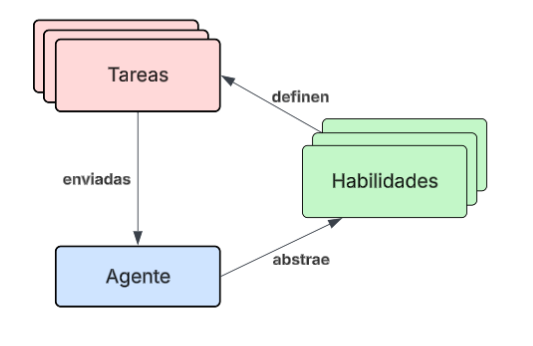
\includegraphics[width=0.9\textwidth]{images/marco-teorico/curr-1}
		\caption{Currículo de habilidad}
		\label{fig:curr-1}
	\end{subfigure}
	\hspace{0.05\textwidth}
	\begin{subfigure}[b]{0.35\textwidth}
		\centering
		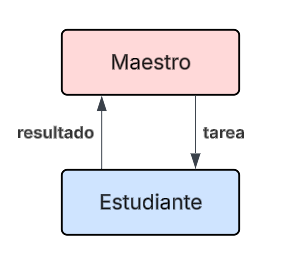
\includegraphics[width=0.7\textwidth]{images/marco-teorico/curr-2}
		\caption{Currículo estudiante-maestro}
		\label{fig:curr-2}
	\end{subfigure}
	
	\vspace{1em}
	
	% Segunda fila
	\begin{subfigure}[b]{0.35\textwidth}
		\centering
		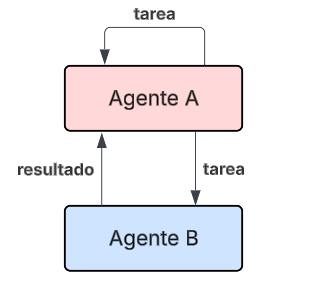
\includegraphics[width=0.65\textwidth]{images/marco-teorico/curr-3}
		\caption{Currículo por Self-Play}
		\label{fig:curr-3}
	\end{subfigure}
	\hspace{0.05\textwidth}
	\begin{subfigure}[b]{0.35\textwidth}
		\centering
		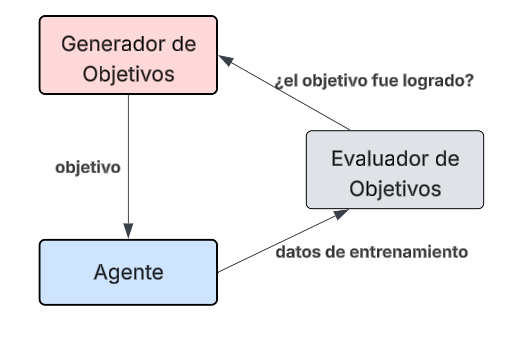
\includegraphics[width=0.9\textwidth]{images/marco-teorico/curr-4}
		\caption{Generación de objetivos automática}
		\label{fig:curr-4}
	\end{subfigure}
	
	\caption{Esquema ilustrativo de los tipos de currículo principales presentados por \textcite{weng2020curriculum}. Las entidades en rojo se encargan de la creación del currículo y las azules entrenan sobre la política de interés.}
	\label{fig:curriculum-types}
\end{figure}


\subsection{Proximal Policy Optimization (PPO)}

PPO es un algoritmo de la familia de gradiente de política, de tipo on-policy introducido por \textcite{schulman2017ppo}. Como otros métodos de la misma familia, PPO mantiene una política estocástica parametrizada $\pi_\theta(a|s)$ y utiliza iterativamente el algoritmo de gradiente ascendente para maximizar la recompensa esperada. La diferencia de PPO es su función objetivo con recorte (llamada Clipping Function), que permite realizar múltiples actualizaciones sobre el mismo conjunto de datos sin que la política nueva se desvíe demasiado de la anterior. En cada paso de actualización de PPO se calcula la relación de probabilidad

$$
r_t(\theta) \;=\; \frac{\pi_\theta(a_t|s_t)}{\pi_{\theta_{\text{old}}}(a_t|s_t)},
$$

y la ventaja estimada $\hat A_t$. El objetivo con recorte está dado por

$$
L^{\mathrm{CLIP}}(\theta) \;=\; \mathbb{E}_t\Big[\min\big(r_t(\theta)\,\hat A_t,\;\mathrm{clip}(r_t(\theta),1-\epsilon,1+\epsilon)\,\hat A_t\big)\Big],
$$

donde $\epsilon>0$ es un parámetro pequeño. Esta formulación recompensa el cambio de política que aumenta la probabilidad de acciones con ventaja positiva, pero impone un límite fijo $(1\pm \epsilon)$ a la relación de probabilidad para evitar grandes saltos de política \parencite{schulman2017ppo}.\\

El algoritmo se puede describir mediante el siguiente pseudocódigo \parencite{schulman2017ppo}:

\begin{algorithm}
	\caption{Proximal Policy Optimization (PPO)}\label{alg:ppo}
	\begin{algorithmic}[1]
		\For {$\text{iteración}=1,2,...$}
		\For {$\text{actor}=1,2,...,N$}
		\State $\text{Ejecutar la política } \pi_{\theta_\text{old}} \text{ en el entorno durante } T \text{ timesteps}$
		\State $\text{Calcular los estimadores de ventaja } \hat{A}_1, ..., \hat{A}_{T}$
		\EndFor
		\State $\text{Optimizar el surrogado } L \text{ respecto a } \theta \text{, con } K \text{ épocas y tamaño de MiniBatch } M \leq NT$
		\State $\theta_{old} \leftarrow \theta$
		\EndFor
	\end{algorithmic}
\end{algorithm}


\subsection{Soft Actor-Critic (SAC)}

Soft Actor-Critic es un algoritmo off-policy de tipo actor-crítico desarrollado por \textcite{haarnoja2018sac}. SAC emplea una política estocástica continua $\pi_\theta(a|s)$ y dos funciones de valor $Q_{\phi_1}(s,a)$ y $Q_{\phi_2}(s,a)$ para mayor estabilidad. Su característica principal es incorporar un término de entropía máxima. El actor maximiza tanto la recompensa esperada como la entropía de la política, lo cual favorece la exploración continua \parencite{haarnoja2018sac}. En la práctica, la política se entrena para maximizar el objetivo. Equivalente a esto, en cada paso de actualización se realiza descenso de gradiente para maximizar el valor esperado de este. \\

Por otro lado, las redes $Q_{\phi_i}$ se actualizan mediante regresión TD utilizando el objetivo de Bellman suavizado por entropía. y se minimiza el error cuadrático de la función Q en ambas redes \parencite{haarnoja2018sac}. A esta técnica de suavizado en los pasos de actualización se le denomina soft updates y son lo que da nombre al algoritmo. En resumen, SAC combina aprendizaje off-policy con un término de entropía en el actor y el critico, logrando actualizaciones estables y eficiente exploración \parencite{haarnoja2018sac}. \\

El algoritmo se puede describir mediante el siguiente pseudocódigo \parencite{haarnoja2018sac}:

\begin{algorithm}
	\caption{Soft Actor-Critic (SAC)}\label{alg:sac}
	\begin{algorithmic}[1]
		\State $\text{Inicializar vectores de parámetros } \psi, \bar{\psi}, \theta, \phi$
		\For {cada iteración}
		\For {cada paso del entorno}
		\State $\mathbf{a}_t \sim \pi_\phi (\mathbf{a}_t|\mathbf{s}_t)$
		\State $\mathbf{s}_{t+1} \sim p(\mathbf{s}_{t+1}|\mathbf{s}_t,\mathbf{a}_t)$
		\State $\mathcal{D} \leftarrow \mathcal{D} \cup \{\mathbf{s}_t,\mathbf{a}_t,r(\mathbf{s}_t,\mathbf{a}_t),\mathbf{s}_{t+1}\}$
		\EndFor
		\For {cada paso del gradiente}
		\State $\psi \leftarrow \psi - \lambda_V \hat{\nabla}_\psi J_V(\psi)$
		\State $\theta_i \leftarrow \theta_i - \lambda_Q \hat{\nabla}_{\theta_i} J_Q(\theta_i) \text{ para } i\in{1,2}$
		\State $\phi \leftarrow \phi - \lambda_\pi \hat{\nabla}_\phi J_\pi(\phi)$
		\State $\bar{\psi} \leftarrow \tau\psi + (1-\tau)\bar{\psi}$
		\EndFor
		\EndFor
	\end{algorithmic}
\end{algorithm}


\subsection{Problema de Cinemática Inversa en Robótica}

La cinemática inversa (IK) es el problema de calcular las posiciones articulares de un manipulador que permiten al efector final alcanzar una orientación y posición deseadas en el espacio. En otras palabras, dada una meta $\mathbf{x}^*$ para el efector final, se busca el vector de ángulos articulares $\mathbf{q}$ tal que $f(\mathbf{q})=\mathbf{x}^*$, donde $f$ es la función cinemática directa. Este problema suele ser no lineal y multivariable \parencite{elhussieny2017inverse}. \\

A nivel matemático, es posible plantear el problema de IK general tomando como base los principios geométricos de la cinemática directa, la cual estudia la determinación de posiciones cartesianas partiendo de los valores de los ángulos articulares conocidos. Esto se logra por medio de la definición de matrices de transformación de coordenadas cartesianas:

$$H = \begin{bmatrix}
	R_n^0 & o_n^0 \\
	\mathbf{0} & 1
	\end{bmatrix}
$$

donde $R_n^0$ es una matriz de rotación acumulada a lo largo de los ejes cartesianos y $o_n^0$ es una matriz de traslación espacial. Se agrega una cuarta columna para mantener la consistencia dimensional y la escala en caso de ser necesaria, pero por defecto es unitaria. Así pues, el problema de IK es equivalente matemáticamente a encontrar una solución del vector $(q_1, q_2, ..., q_n)$ que satisfaga la ecuación:

\begin{equation}
	T_n^0(q_1, q_2, ..., q_n) = A_1(q_1) A_2(q_2) ... A_n(q_n) = H
\end{equation}

Adicionalmente, cabe resaltar que los manipuladores redundantes (aquellos que tienen más de 6 DOF) pueden tener infinitas soluciones, mientras que en posiciones singulares como articulaciones alineadas la solución puede no existir o ser inestable \parencite{elhussieny2017inverse}. Robots complejos como Pepper ejemplifican esta dificultad pues cuenta con una base omnidireccional de 3 DOF, torso con 3 DOF, cabeza 2 DOF y cada brazo 5 DOF (más dedos), sumando alrededor de 18 DOF totales \parencite{softbank2023pepper}. La alta redundancia de Pepper implica infinitas configuraciones articulares para una misma posición del efector, y además la cinemática no admite una solución analítica sencilla en general.\\

\subsubsection{Métodos clásicos de solución de IK}

Los métodos clásicos para resolver cinemática inversa suelen basarse en aproximaciones numéricas del jacobiano o soluciones analíticas parciales. Entre ellos destacan: 

\begin{itemize}
	\item \textbf{Método del jacobiano inverso}: ajusta iterativamente los ángulos articulares usando la pseudoinversa del jacobiano para acercar el efector a la posición deseada.
	
	\item \textbf{Método del jacobiano transpuesto o de gradiente}: emplea la transpuesta del jacobiano como dirección de corrección, similar a un descenso de gradiente clásico.
	
	\item \textbf{Métodos de mínimos cuadrados amortiguados}: introduce un término de regularización para mejorar la estabilidad en configuraciones cercanas a singularidades \parencite{zhao2024inverse}.
\end{itemize}


También se encuentran soluciones analíticas geométricas en robots especiales (métodos algebraicos basados en transformaciones de coordenadas), pero son poco generales. En la práctica, estas técnicas requieren cuidadosa sintonización de parámetros como pasos de actualización o criterios de convergencia, y pueden tener dificultades cerca de singularidades o límites articulares.\\

\subsubsection{Métodos basados en RL para solución de IK}

En contraste, los enfoques de aprendizaje automático y reforzado evitan formular explícitamente la cinemática y aprenden directamente políticas o modelos para alcanzar la meta. Por ejemplo, existen propuestas de algoritmos como MAPPO-IK, el cual está basado en PPO, para un manipulador de 6 DOF. En este escenario, el diseño del agente RL fue elaborado para recibir la diferencia de posición esperada-calculada como recompensa de cada paso \parencite{zhao2024inverse}. De manera similar, se ha propuesto el entrenamiento de un agente sobre un simulador de robot humanoide para resolver la cinemática inversa mediante una política similar, pero de carácter estocástico a la hora de definir la recompensa \parencite{adjei2024safe}.\\ 

De igual manera, se han planteado desarrollos que emplean redes neuronales profundas (Aprendizaje por Refuerzo Profundo) para aprender la relación inversa de un manipulador sin necesidad de calcular explícitamente las matrices jacobianas \parencite{liu2021deep}. En general, estas soluciones basadas en RL pueden adaptarse mejor a entornos dinámicos o restricciones complejas (posturas factibles, colisiones), aunque suelen requerir entrenamiento previo intensivo. Además del RL directo para IK, la literatura reciente destaca dos aproximaciones distintas. En particular, conviene mencionar trabajos que combinan aprendizaje reforzado con restricciones de seguridad y razonamiento de recompensas para garantizar trayectorias seguras en brazos robóticos \parencite{ozalp2024advancements}. \\

Por último, en la misma línea de los algoritmos propios del RL, se han desarrollado enfoques basados en Deep Q-Networks (DQN) para resolver la cinemática inversa de un manipulador de 7 DOF, usando la formulación de Producto de Exponenciales (PoE) para la cinemática directa y generando trayectorias articulares discretas con alta estabilidad frente a la sensibilidad de hiperparámetros típica de métodos continuos \parencite{malik2022deeprl}. Estos trabajos ilustran cómo tanto la revisión estructurada del estado del arte como la aplicación práctica de RL pueden avanzar la resolución de IK en manipuladores complejos.\\
